\section{Anpassungsphase}

\begin{figure}[htbp] 
	\centering
	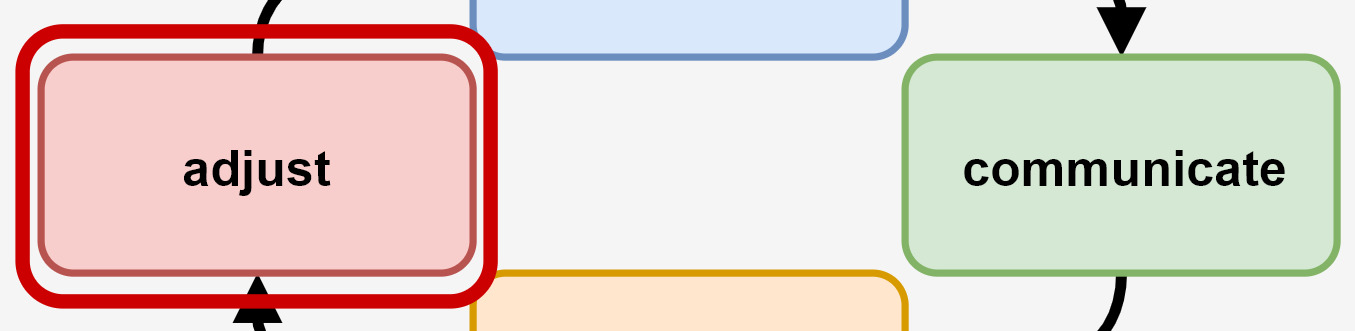
\includegraphics[width=0.75\textwidth]{contents/images/SmartGrazerSectionAdjust}
	\caption{SmartGrazer: Auszug Anpassungsphase}
	\label{fig:SmartGrazerSectionAdjust}
\end{figure}

Nach der Analysephase wird, sofern kein gültiger Payload gefunden wurde, die Liste der veränderten Elemente zurück an den Smarty-Generator übergeben. Dieser aktualisiert seine Element-Datenbank und generiert anhand der neuen Lebenspunkte weitere Payloads. Im Folgenden wird erläutert, wie die Gewichtung bei der Payload-Generierung implementiert wurde.

\subsection{Gewichtung der Elemente}\label{ssec:elementlifepoints}

Durch eine Gewichtung der Elemente lässt sich die Wahrscheinlichkeit, dass ein Element erneut gezogen wird, beeinflussen. Dementsprechend ist gewollt, dass entfernte oder veränderte Bestandteile von Payloads weniger häufig gewählt werden. Anhand der Gewichtung lässt sich im weiteren Verlauf das Potential eines Payloads errechnen. Dies hat zur Folge, dass Payloads quantitativ vergleichbar werden.

%Als Gewichtung wird ein Attribut definiert, welches abbildet, wie wahrscheinlich es ist, dass ein Element im generierten Payload verwendet wird. 
Für die Generierung wird ein zusätzliches Attribut definiert. Dieses bildet die Wahrscheinlichkeit ab, dass ein Element im generierten Payload verwendet wird. Bezeichnet wird dieses Attribut im weiteren Verlauf als das Leben eines Elements. Wie bereits gezeigt, kann zum Beispiel das ``SPACE''-Element verschiedene Werte annehmen. Werden einige dieser Werte durch die SUT gefiltert oder verändert, soll der Generator die nicht geänderten Elemente priorisieren. Die Implementierung dieser priorisierten Ziehung wird in Kapitel \ref{ssec:weightedRandom} näher erläutert.

Bei der Initialisierung wird der Wert des Attributs auf eine Größe von maximal 100 Lebenspunkten  gesetzt. Zusätzlich ist definiert, dass das Leben eines Elements nicht unter eins fallen kann. Die Festlegung der oberen Grenze stellt zum Einen sicher, dass zu jedem Zeitpunk der Ausführung das maximale Potential einer Angriffsgrammatik bestimmt werden kann. Zum Anderen wird durch das Festlegen der unteren Grenze sichergestellt, dass kein Element aus der Generierung ausgeschlossen wird. Dies ist bei schlecht implementierten WAF vorteilhaft, weil diese komplette Zeichenketten, wie zum Beispiel ``\lstinline[language=html]!<script>!'' oder ``\lstinline[language=html]!</script>!'', aus Benutzereingaben herausfiltern. Durch das Erhalten von einem Lebenspunkt wird sichergestellt, dass die einzelnen Elemente \lstinline[language=html]!``<'', ``/'', ``script''! oder \lstinline[language=html]!``>''! auch in anderen Angriffsmustern wiederverwendet werden können. Ein entsprechendes Beispiel wird in Abbildung \ref{fig:SmartGrazerWeightedElementsKeepOne} gezeigt. In diesem Beispiel besteht die Element-Datenbank aus den Elementen im gelben Bereich. Durch das Senken der Lebenspunkte des Schrägstrich-Zeichens auf Null, werden dem oberen Payload dringend benötigte Elemente genommen.

\begin{figure}[htbp] 
	\centering
	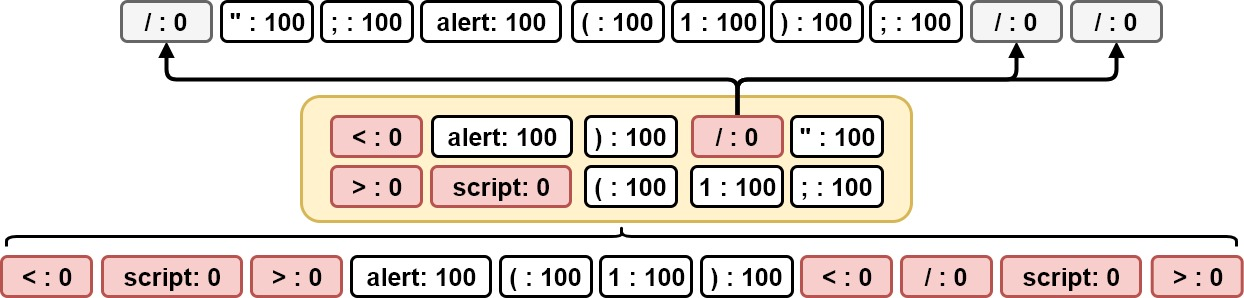
\includegraphics[width=\textwidth]{contents/images/SmartGrazerWeightedElementsKeepOne}
	\caption{SmartGrazer: Auswirkungen auf die Lebenspunkte}
	\label{fig:SmartGrazerWeightedElementsKeepOne}
\end{figure}

\begin{figure}[htbp] 
	\centering
	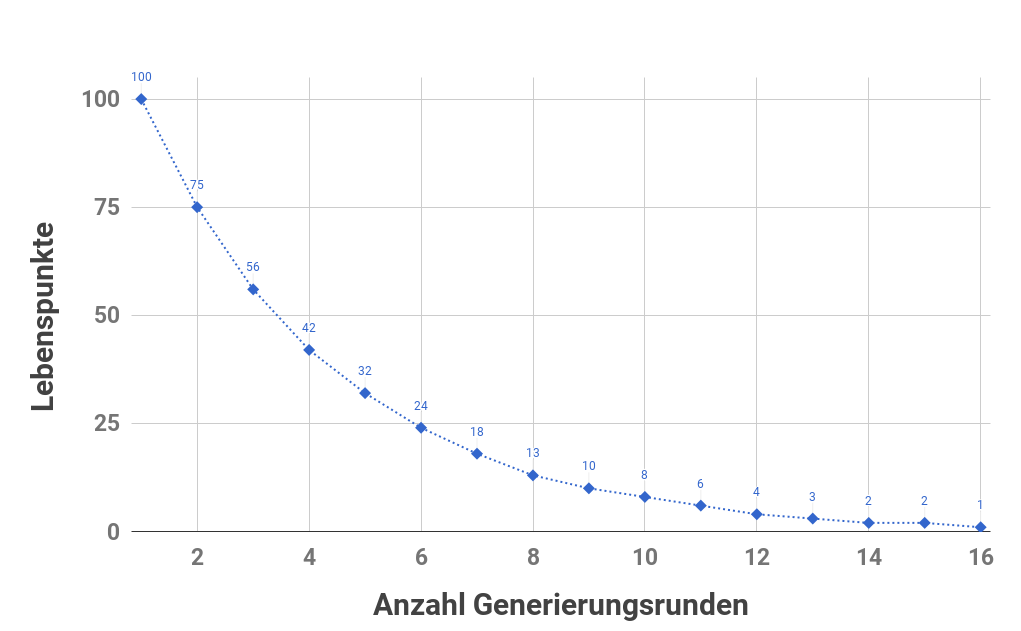
\includegraphics[width=\textwidth]{contents/images/ElementsDecreasingLifepoints}
	\caption{SmartGrazer: Verlauf der Lebenspunkte pro Senkung}
	\label{fig:decreasing-Lifepoints}
\end{figure}

In Abbildung \ref{fig:decreasing-Lifepoints} ist abgebildet, wie sich die Lebenspunkte bei einem Faktor von 0,75 verringern. Der Faktor bewirkt, dass die Lebenspunkte nach den ersten drei Generierungsrunden unter 50\% fallen, insgesamt jedoch 16 Runden nötig sind um die Lebenspunkte auf eins zu senken.

\FloatBarrier

\paragraph{Beispiel:} Um ein näheres Verständnis von der Funktionsweise der Gewichtung zu bekommen, wird Anhand der Abbildung \ref{fig:SmartGrazer-adjustmentExample} ein konstruiertes Beispiel betrachtet. In dem gezeigten Beispiel hat Smarty nur eine Payload-Definition zur Verfügung, damit die Veränderung der generierten Payloads nachvollzogen werden können. Das \ac{SUT} filtert alle doppelten und einfachen Anführungszeichen aus Benutzereingaben heraus, weitere Veränderungen an den Eingaben werden nicht vorgenommen.

Bei der ersten Generierungsrunde wurden alle Elemente mit 100 Lebenspunkten initialisiert und an SmartGrazer übergeben. Smarty generiert daraufhin einen Payload, der drei verschiedene Arten von Anführungszeichen enthält. Bei der Analyse ermittelt SmartGrazer die gefilterten Elemente und verringert deren Lebenspunkte wie in diesem Kapitel beschrieben.

In der zweiten Runde werden die gefilterten Elemente ebenfalls im Payload verwendet und wiederholt herausgefiltert.

\begin{figure}[htbp] 
	\centering
	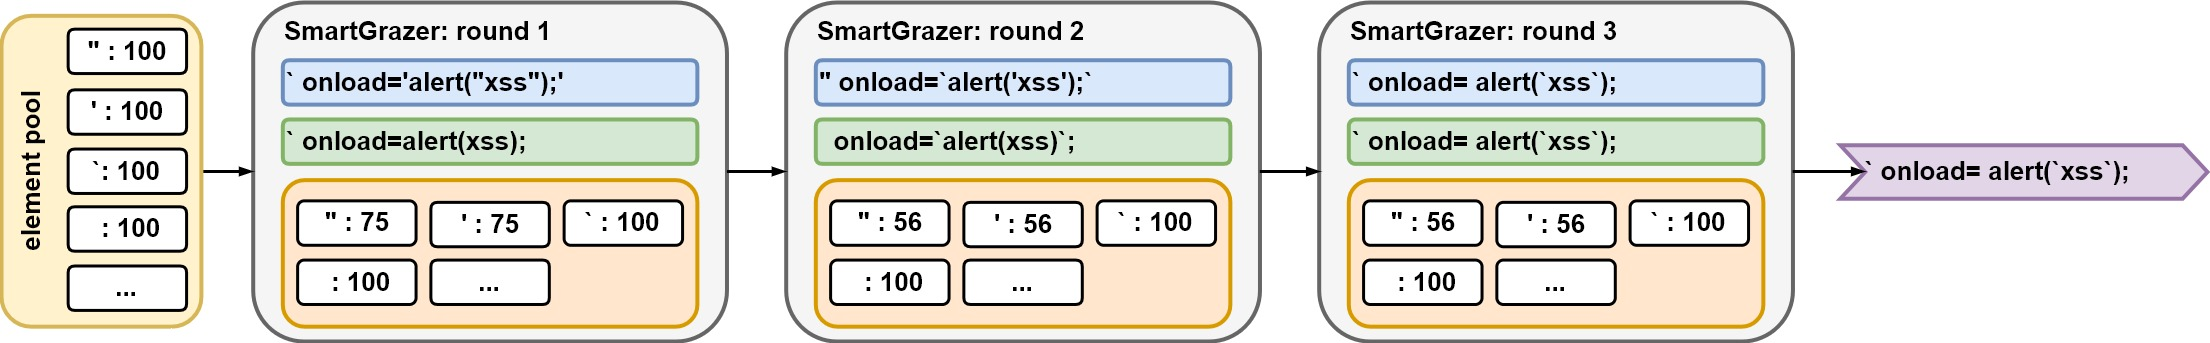
\includegraphics[width=\textwidth]{contents/images/SmartGrazerAdjustmentExample}
	\caption{Beispiel: Gewichtung von Elementen}
	\label{fig:SmartGrazer-adjustmentExample}
\end{figure}

Für die letzte Runde werden Anführungszeichen verwendet, deren Lebenspunkte nicht verringert worden sind. Da keine Elemente verändert wurden, beendet SmartGrazer die Generierung und gibt den gefundenen Payload zurück.

\FloatBarrier
\subsubsection{Payload-Potentiale:}

Das Potential eines Payloads setzt sich aus der Summe der Lebenswerte seiner enthaltenen Elemente zusammen. Hierbei wird zunächst die Summe der maximalen Leben errechnet. Anschließend wird der tatsächliche Lebenswert aller Elemente zusammengezählt. Durch Division der beiden Werte, wie in Abbildung \ref{fig:payloadgrammarpotential} dargestellt, errechnet sich das Potential des Payloads. Gegeben sind die Elemente der Payload-Zeichenkette: \lstinline[language=html]!"><a\tonclick =alert\v('53')>)!. Hierbei wird das maximale Leben des Payloads mit der Formel \lstinline[language=html]!maxLife = 100 * sum(elements)! berechnet. Das tatsächliche Leben der enthaltenen Elemente errechnet sich durch einfaches aufaddieren der Lebenspunkte. Im gegebenen Beispiel ergeben sich dementsprechend die Werte \lstinline[language=html]!maxLife = 1600! und \lstinline[language=html]!currentLife = 1363!. Mittels einer Division der beiden Werte errechnet sich dann das Potential des Payloads. Im aktuellen Beispiel beträgt dieser \lstinline[language=html]!0,85! (gerundet). Dieser Wert wird während der Generierung errechnet und mit dem anderer Payloads verglichen, sodass aus mehreren Payloads der am besten geeignete Kandidat an die Webseite gesendet wird.

\begin{figure}[htbp] 
	\centering
	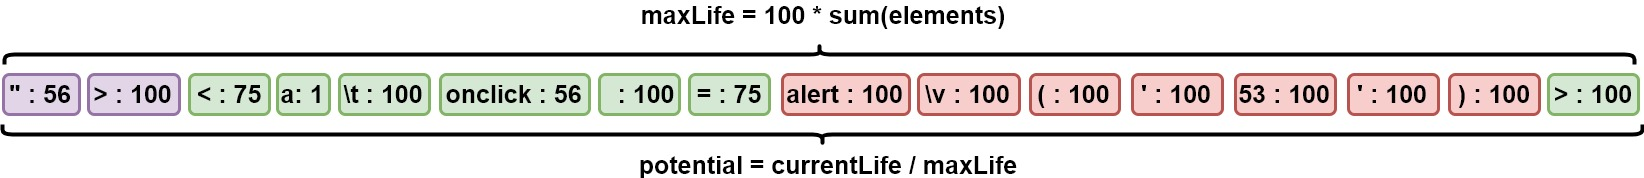
\includegraphics[width=\textwidth]{contents/images/PayloadGrammerPotential.jpg}
	\caption{Beispiel: Errechnung des Payload-Potentials}
	\label{fig:payloadgrammarpotential}
\end{figure}


\subsubsection{Wahl eines Payloads mit größtem Erfolgspotential:}

Smarty erstellt in jeder Generierungsrunde zunächst drei Payloads aus den verfügbaren Mustern und errechnet den Payload mit dem größten Potential, wie in Abbildung \ref{fig:payloadgrammarpotential} dargestellt. Ein Struktogramm des Algorithmus ist in Abbildung \ref{fig:StructoGetWithMostPotential} dargestellt.

\begin{figure}[htbp] 
	\centering
	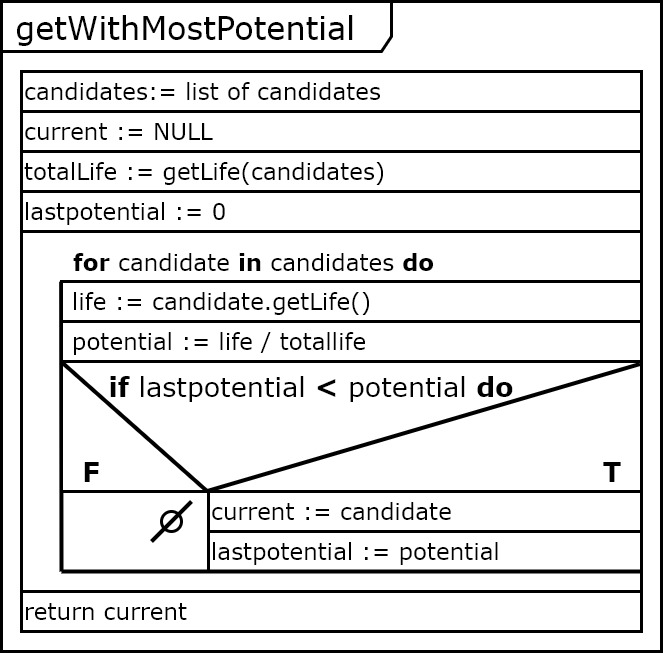
\includegraphics[width=.62\textwidth]{contents/images/StructoGetWithMostPotential}
	\caption{Struktogramm: getWithMostPotential}
	\label{fig:StructoGetWithMostPotential}
\end{figure}

\subsubsection{Gewichteter Zufall bei Elementen}\label{ssec:weightedRandom}

Bei allen Elementen mit mehreren möglichen Zeichen bzw. Zeichenketten, wie zum Beispiel den HTML-Tags oder Events, wird eine gewichtete Zufallsziehung durchgeführt, wie im Struktogramm \ref{fig:StructoPickWeightedRandom} dargestellt.

\begin{figure}[htbp] 
	\centering
	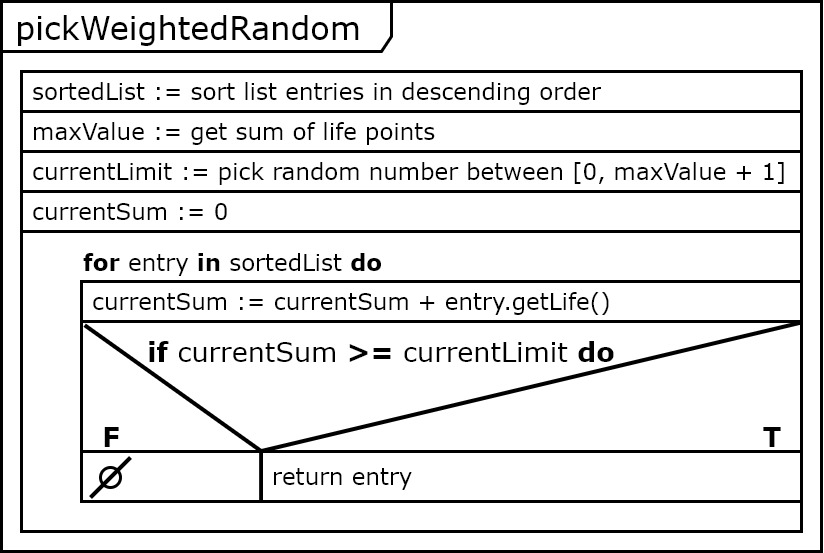
\includegraphics[width=0.80\textwidth]{contents/images/StructoPickWeightedRandom}
	\caption{Struktogramm: pickWeightedRandom}
	\label{fig:StructoPickWeightedRandom}
\end{figure}

\FloatBarrier
In Abbildung \ref{fig:SmartGrazer-weightedRandomExample} ist ein konstruiertes Beispiel mit niedrigen Lebenspunkten abgebildet. Gegeben sind drei Elemente für Anführungszeichen mit jeweils einem, zwei und drei Lebenspunkten. Der Algorithmus sortiert zunächst alle Einträge einer Liste absteigend anhand der Lebenspunkte und berechnet anschließend, wie viel Lebenspunkte alle Elemente der gegebenen Liste zusammen enthalten. Im nächsten Schritt wird eine zufällige Zahl zwischen 0 und einschließlich der maximalen Lebenspunktezahl + 1 errechnet.

Zuletzt wird die Liste durchlaufen und die ``currentSum''-Variable um den Wert der Lebenspunkte des aktuellen Elements erhöht. Sobald ``currentSum'' größer oder gleich groß ist, wie der zufällig gezogene Wert, wird das aktuelle Element zurückgegeben.

\begin{figure}[htbp] 
	\centering
	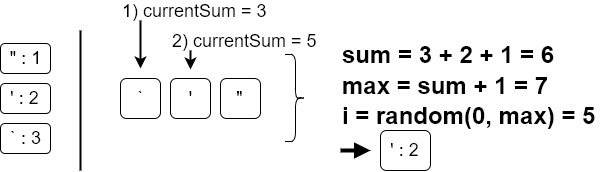
\includegraphics[width=0.60\textwidth]{contents/images/SmartGrazerWeightedRandomExample}
	\caption{Beispiel: Gewichtete Zufallsziehung }
	\label{fig:SmartGrazer-weightedRandomExample}
\end{figure}